\documentclass[../main.tex]{subfiles}
\begin{document}
\part*{Infrastructure}
The infrastructure described is a common architecture for building web applications that require image classification capabilities. The infrastructure is divided into two tiers: the Web-Tier and the Application-Tier.

The Web-Tier of the system consists of a simple User Interface, where a user can interact with our system. In our system, user can upload images they want to classify. The Application-Tier contains core functionality of the system, image classification. It also handles business logic, database manipulation functions (CRUD), and communicates with other resources. The overall system architecture of our project can be viewed in the Figure~\ref{fig:arc}.

\begin{figure}[h!]
\centering
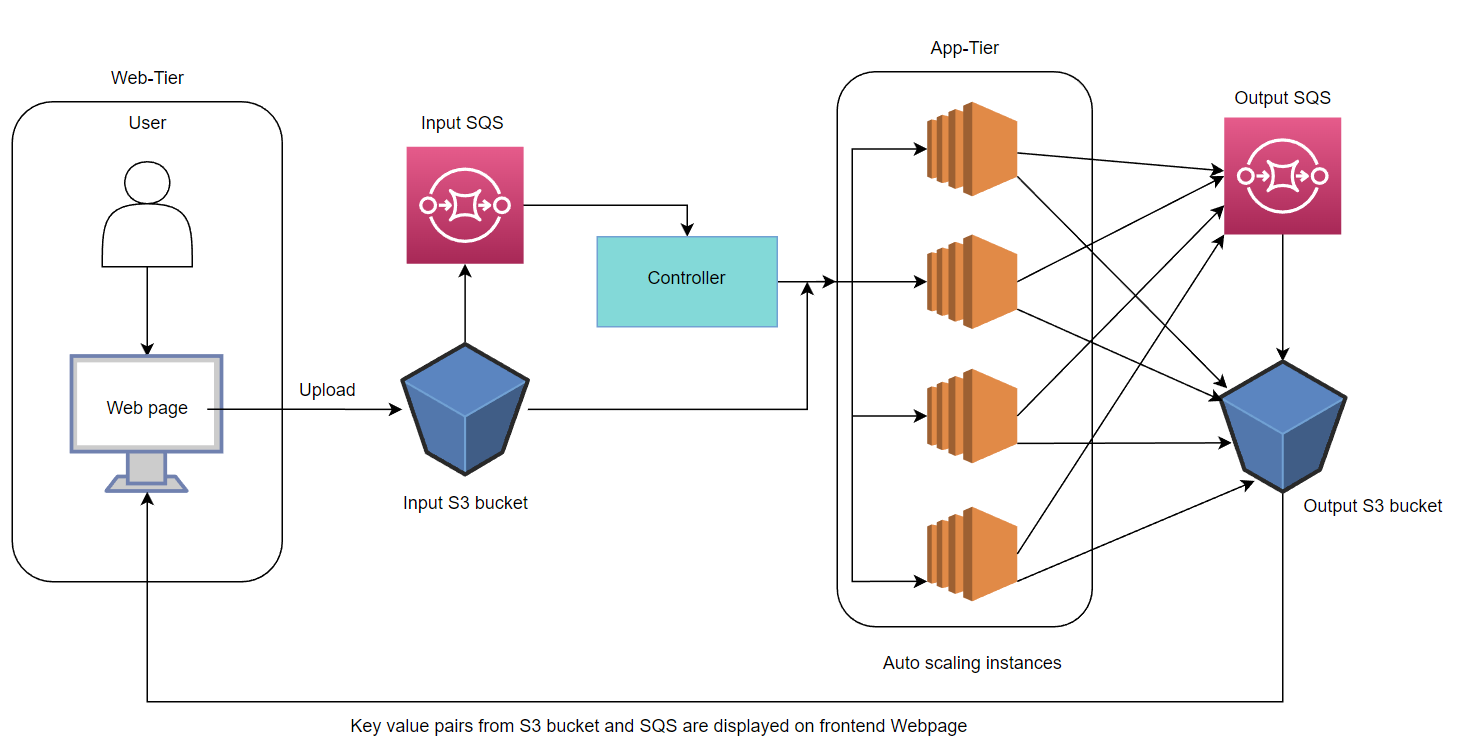
\includegraphics[scale=0.68]{images/arc.png}
\caption{System Architecture.}
\label{fig:arc}
\end{figure}

The number of EC2 instances needed depends on the frequency of data uploads. Scaling in and scaling out of instances are determined based on the number of input images uploaded, which are fed into the SQS queue and the number of messages are calculated. Scaling in is managed by the controller, which automatically terminates instances when there are no more messages left in the input SQS. Scaling out is implemented using the number of running instances and the estimated number of visible SQS messages. Instances are created with the AMI, and the scaling out logic is designed not to create more than 15 instances. To summarize, the number of instances created depends on the number of SQS messages. If there are less than 15 messages, the number of instances created will be the number of messages minus the number of currently running instances. If there are more than 15 messages, 17 instances will run to handle the increased load and avoid errors during the processing of larger images.

This infrastructure utilizes AWS' EC2, SQS, and S3 resources. Specifically, the App Tier relies on S3 and SQS to store and transmit data, respectively. Once the classification results are generated, they are sent as key-value pairs to the output SQS and output S3 bucket to be displayed on the web page.

The infrastructure is a standard two-tier architecture used to develop web applications that incorporate image classification features. The Web-Tier provides a user interface for uploading images, while the Application-Tier contains core functionality, such as image classification, business logic, and database manipulation functions. AWS EC2, SQS, and S3 resources are utilized to create this infrastructure. Scaling in and out of resources is determined by the number of incoming images, which are processed through SQS, and the number of running instances. The infrastructure is designed to create up to 15 instances, and the number of instances created is based on the number of incoming images, with automatic termination of instances when the queue is empty. By leveraging AWS services and this scalable infrastructure, web applications with image classification capabilities can be built in a cost-effective and efficient manner.
% Overall, this infrastructure provides a scalable and cost-effective way to build web applications with image classification capabilities. By separating the Web and Application Tiers and using AWS services, the infrastructure can automatically scale resources up or down based on demand, improving performance and reducing costs.

\end{document}

\clearpage